\section{The important of AVAILABLE object in linear probing for Hash-tables}

\subsection{Instruction}
Assume the utilization of linear probing for hash-tables. To enhance the complexity of the
operations performed on the table, a special AVAILABLE object is used. Assuming that all keys
are positive integers, the following two techniques were suggested in order to enhance complexity:
\begin{itemize}
    \item 
\item[] i) In case an entry is removed, instead of marking its location as AVAILABLE, indicate
the key as the negative value of the removed key (i.e. if the removed key was 16,
indicate the key as -16). Searching for an entry with the removed key would then
terminate once a negative value of the key is found (instead of continuing to search if
AVAILABLE is used).

\item[] ii) Instead of using AVAILABLE, find a key in the table that should have been placed in
the location of the removed entry, then place that key (place the entire entry of course)
in that location (instead of setting the location as AVAILABLE). The motive is to find
the key faster since it is now in its hashed location. This would also avoid the
dependence on the AVAILABLE object.
\end{itemize}
Will either of these proposals enhance the search time complexity? Additionally, will any of these
approaches result in misbehaviour (in terms of functionalities, or even performance)? If so, explain
clearly through illustrative examples. 

\subsection{Claim:}
\textbf{In this particular problem, since the statement indicates the sign of interchange in keywords "key" and "hash-value", the answer for this also assumes the interchanging of these two keywords. However, the distinction in the keywords is still important to be recognized in order to avoid any further confusion. "Key" is usually referred to an entry in a pair of element (key, value), while "hash-value" is usually the integer value of a key after being hashed by a function. In this problem, to whom read this, please perceive the term "key" as in fact, "hash value". }

\subsection{Consider alternative method I}
The first proposal will not change the \textit{search} time complexity at all since the algorithm still has to iterate through all the probes, and eventually reaches the \textbf{recent removed entry} with negative value. Thus, the time complexity for \textit{search} operation is still \textbf{O(n)}, which means it does not improve anything.
\\
Moreover, there is a high chance the algorithm will \textbf{misbehaviour} in many situations. 
\\
\textbf{Consider the following situation:}
\\
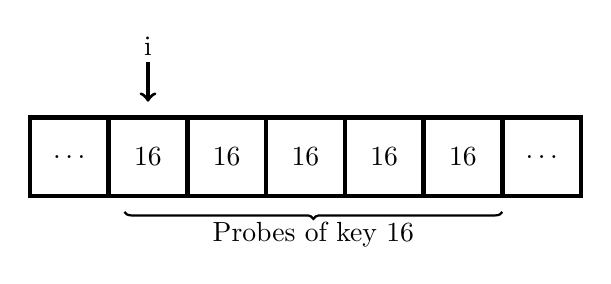
\begin{tikzpicture}
    [%%%%%%%%%%%%%%%%%%%%%%%%%%%%%%
        box/.style={rectangle,draw=black, ultra thick, minimum size=1cm},
    ]%%%%%%%%%%%%%%%%%%%%%%%%%%%%%%
\foreach \x/\y in {0/\text{$\dots$},1/16,2/16,3/16,4/16,5/16,6/\text{$\dots$}}
        \node[box] at (\x,0){\y};

\draw[decorate,decoration={brace,mirror},thick] (0.7,-.7) -- node[below]{Probes of key 16} (5.5,-.7);
\draw[->,very thick] (1,1.2) --  node[above,yshift=2mm]{i} (1,.7);

\end{tikzpicture}
\\
\textbf{Remove A[i]. Then as proposed, replace the key with negative value.}
\\
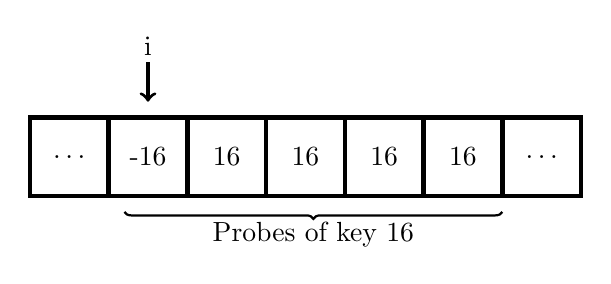
\begin{tikzpicture}
    [%%%%%%%%%%%%%%%%%%%%%%%%%%%%%%
        box/.style={rectangle,draw=black, ultra thick, minimum size=1cm},
    ]%%%%%%%%%%%%%%%%%%%%%%%%%%%%%%
\foreach \x/\y in {0/\text{$\dots$},1/-16,2/16,3/16,4/16,5/16,6/\text{$\dots$}}
        \node[box] at (\x,0){\y};

\draw[decorate,decoration={brace,mirror},thick] (0.7,-.7) -- node[below]{Probes of key 16} (5.5,-.7);
\draw[->,very thick] (1,1.2) --  node[above,yshift=2mm]{i} (1,.7);

\end{tikzpicture}
\\
In this situation, when using \textit{search} algorithm for key 16, the algorithm will stop at A[i], and return null indicating there is no such key in the array. While in reality, there are plenty of entries with key 16 in the probes after -16. Therefore, the algorithm misses the actual results.
\\
In fact, the algorithm only behaves as expected when there is \textbf{only} one single probe of a key. If that is the case, then it completely defeats the purpose of open-addressing.

\subsection{Consider alternative method II}
This proposed method will make a slightly improvement in \textit{search} operation in the hash-table. However, it may lead to a more serious problem in term of algorithm behaviour. For example:
\\
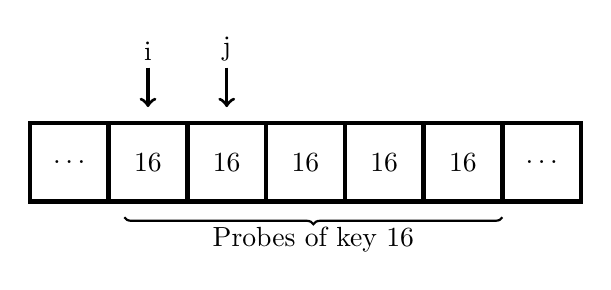
\begin{tikzpicture}
    [%%%%%%%%%%%%%%%%%%%%%%%%%%%%%%
        box/.style={rectangle,draw=black, ultra thick, minimum size=1cm},
    ]%%%%%%%%%%%%%%%%%%%%%%%%%%%%%%
\foreach \x/\y in {0/\text{$\dots$},1/16,2/16,3/16,4/16,5/16,6/\text{$\dots$}}
        \node[box] at (\x,0){\y};

\draw[decorate,decoration={brace,mirror},thick] (0.7,-.7) -- node[below]{Probes of key 16} (5.5,-.7);
\draw[->,very thick] (1,1.2) --  node[above,yshift=2mm]{i} (1,.7);
\draw[->,very thick] (2,1.2) --  node[above,yshift=2mm]{j} (2,.7);

\end{tikzpicture}
\\
\textbf{Removing the first element in the probe. Then found another key to replace the removed position}
\\
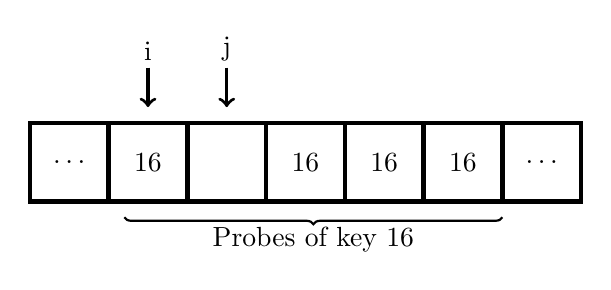
\begin{tikzpicture}
    [%%%%%%%%%%%%%%%%%%%%%%%%%%%%%%
        box/.style={rectangle,draw=black, ultra thick, minimum size=1cm},
    ]%%%%%%%%%%%%%%%%%%%%%%%%%%%%%%
\foreach \x/\y in {0/\text{$\dots$},1/16,2/,3/16,4/16,5/16,6/\text{$\dots$}}
        \node[box] at (\x,0){\y};

\draw[decorate,decoration={brace,mirror},thick] (0.7,-.7) -- node[below]{Probes of key 16} (5.5,-.7);
\draw[->,very thick] (1,1.2) --  node[above,yshift=2mm]{i} (1,.7);
\draw[->,very thick] (2,1.2) --  node[above,yshift=2mm]{j} (2,.7);
\end{tikzpicture}
\\
The \textit{search} operation will terminate at A[j] since it is an empty position (indicating the end of probe). But in fact, there are more elements with the same key after that empty position. Thus, the algorithm misses checking those elements, resulting in a possible lost of searching results. 
\\
However, this problem could be avoided if the algorithm was implemented by checking every position after the first-found possible hashed location. But this results in a time complexity of \textit{O(n)}, which means it does not improve anything. As a matter of fact, the algorithm is even slower in some cases than that using AVAILABLE object. Implementing the mechanism of AVAILABLE object will provide a chance to terminate the algorithm by reaching empty position without having to iterate until the last element in the table.



